\index{Renner, Britta}

\paragraph{Research Team}
Britta Renner (Professor), Freda-Marie Hartung (Doctoral Fellow).

 A first line of research of the Personality Psychology Research Group focuses on interpersonal perception with a particular emphasis on expectancies and curiosity. The goal of this line of research is to determine how people derive judgments of another person, which factors facilitate or diminish the accuracy in personality judgments and how accuracy varies with age. 
A second line of research focuses on the conceptualizing of and reaction towards optimism, pessimism, and realism. Numerous studies have demonstrated that optimism is linked to positive outcomes (e.g., health) by a ``social pathway'' (Peterson \& Bossio, 2001). However, this \
``social pathway'', that is social reactions towards optimism and pessimism, has only rarely been studied. Therefore, the goal of this line of research is to examine whether judges respond differentially to optimism, realism and pessimism, and whether these differential responses can be related to specific cues of optimism, realism and pessimism.

\null
\textbf{Research Highlights 2006}

{\textit{Development of a Measurement of Social Curiosity in Adults}

 Curiosity refers to the desire for acquiring new information. Available measures assess curiosity predominantly in the non-social domain. The aim of the present study was to develop a questionnaire to assess social curiosity, i.e., interest in how other people think, feel and behave. The questionnaire was administered to 312 participants. Factor analyses of the 10-item Social Curiosity Scale (SCS) yielded two factors: (1) General Social Curiosity and (2) Covert Social Curiosity. Evidence of convergent validity was provided by moderately high correlations of the SCS with other measures of curiosity and self-perceived curiosity, while divergent validity was demonstrated by low correlations of the SCS with other personality traits, such as neuroticism and agreeableness. Interestingly, social interaction anxiety was observed to facilitate covert social curiosity while inhibiting general social curiosity (cf., Renner, 2006). Taking a lifelong learning perspective, we were additionally interested in the question, how curiosity or the motivation to learn about our physical and social world varies across the lifespan. In contrast to common stereotypes, curiosity did not decrease with increasing age suggesting that the basic motivation to learn appears to remain stable over the lifespan.

\textit{Conceptualizing of and Social Reaction towards Optimism, Pessimism and Realism}

 Numerous studies have shown that optimism is linked to positive outcomes (e.g., health) by a ``social pathway'' (Peterson \& Bossio, 2001). This research program focuses on the question how lay people perceive typical optimistic, pessimistic and realistic acts (DFG funded research project together with Prof. Dr. Hannelore Weber, University of Greifswald). Using a multidimensional perspective, not only typical behavior and typical thoughts are assessed but also typical feelings and typical goals are considered from an act frequency perspective (Weber, Vollmann, \& Renner, in press). In a second step, this line of research examines reactions to optimistic, realistic and pessimistic prototypical acts. Specifically, two experiments (N = 240 and N = 120) examined social responses toward optimists, pessimists, and realists (Vollmann, Renner, \& Weber, submitted). Participants listened to tape-recorded conversations in which optimistic, pessimistic and realistic targets reported how they were dealing with a stressful situation before completing a questionnaire assessing (a) their evaluation of the target's behavior and personality, (b) their attraction to the target, and (c) their willingness to provide the target with social support. Optimistic and realistic targets were viewed more favorably than pessimistic targets, while the behavior of realists was regarded as being more adequate than that of optimists. However, the more positive evaluation of optimists and realists compared to pessimists was not accompanied by a greater willingness to provide them with social support (see Figure \ref{fig3:profBrittaRenner}). The unequivocally high willingness to provide support to both optimists and pessimists might suggest that optimists are in fact not provided with more social support than pessimists. Accordingly, the greater availability of social support commonly reported by optimists (e.g., Brissette et al., 2002) might represent an optimistically biased perception rather than an accurate reflection of the support they are provided with.

\begin{figure}[ht]
  \begin{center}
    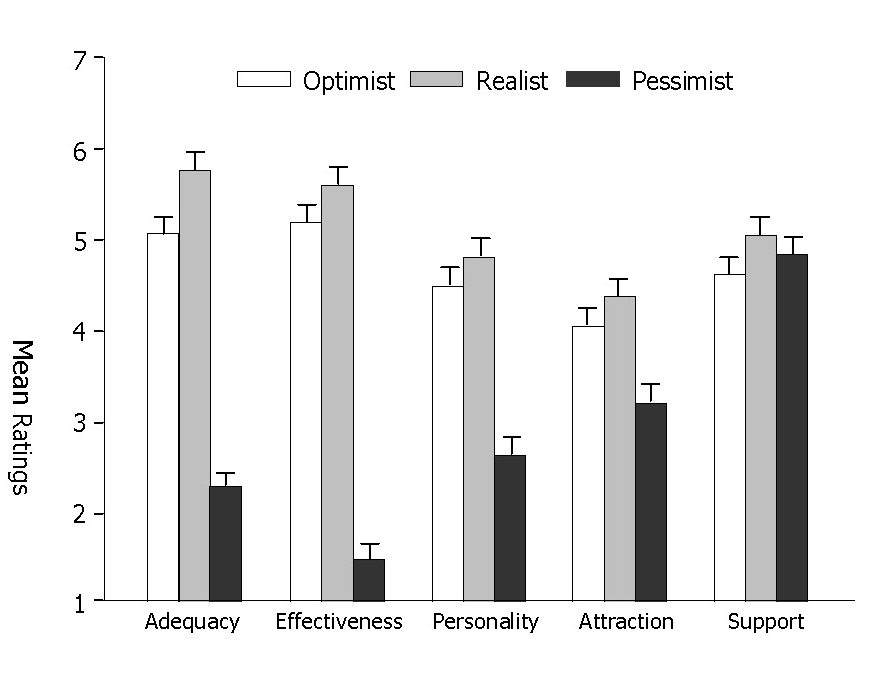
\includegraphics[height=25ex, width=0.5\textwidth]{profBrittaRenner-fig3.jpg}
    \caption{Mean evaluation ratings (with standard errors) of the target as a function of the type of target behavior pattern (Study 2). Note: Higher values indicate a more positive evaluation. (Vollmann, Renner, \& Weber, submitted)}\label{fig3:profBrittaRenner}
   \end{center}
\end{figure}


\textbf{Collaborations}
\begin{itemize}
\item University of Greifswald \\ Prof. Dr. Hannlore Weber; Dipl.-Psych. Manja Vollmann
\item University of Halle \\ Prof. Dr. Peter Borkenau
\end{itemize}

\enlargethispage{1cm}
\begin{bibunit}[apalike]
\nocite{*}
\putbib[profBrittaRenner2]
\end{bibunit}